\subsection{Inversion--recovery}
\label{subsec:poise__invrec}


\subsubsection{Optimisation setup}

\begin{figure}[htb]
    \centering
    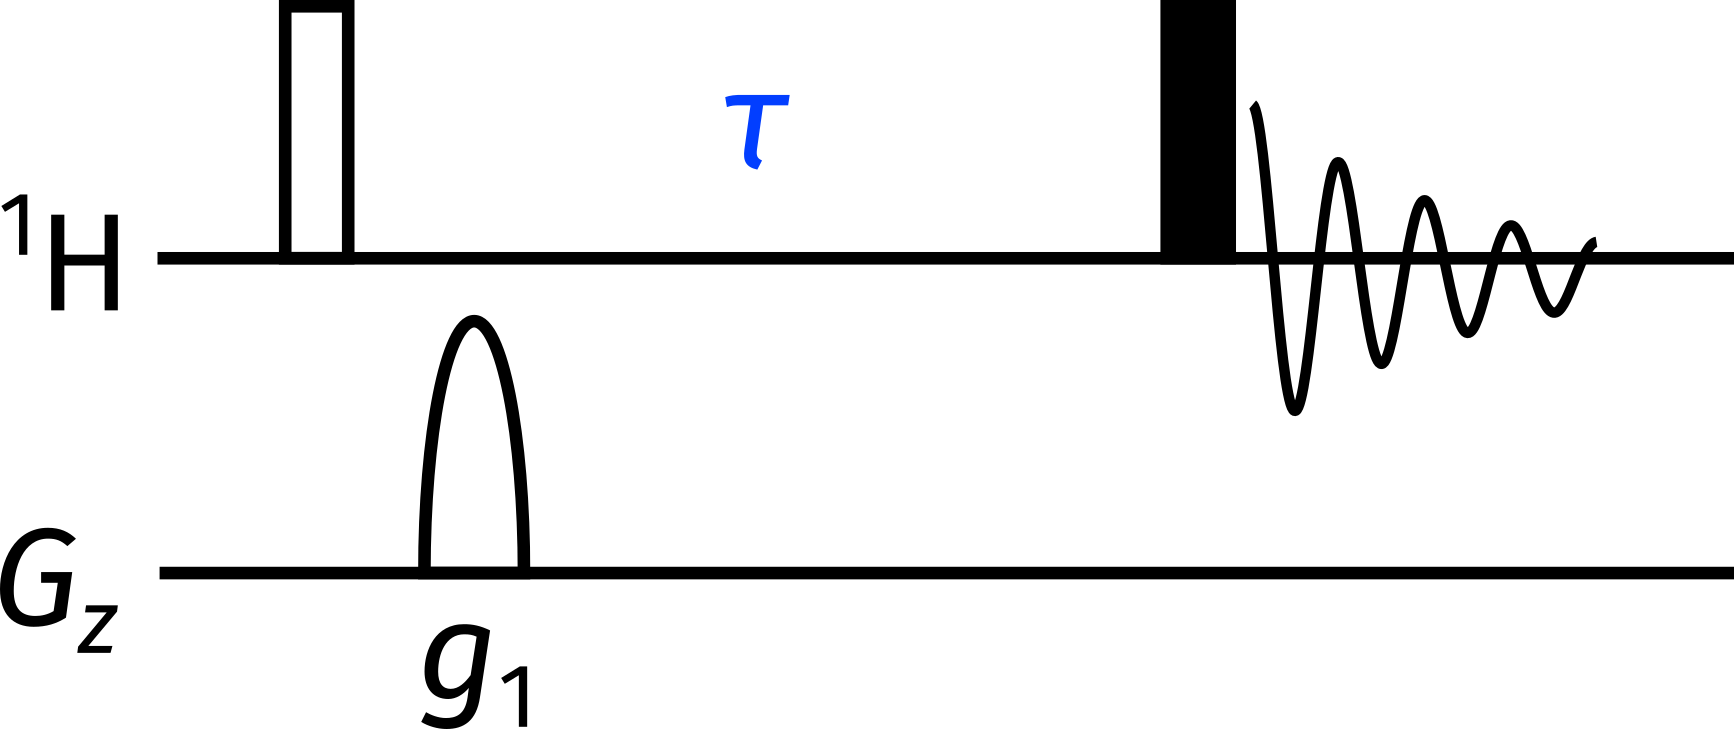
\includegraphics[]{pp/poise/invrec.png}%
    \caption[Inversion--recovery pulse sequence]{Inversion--recovery pulse sequence.}
    \label{fig:poise_invrec}
\end{figure}

If what we really want to measure is $T_1$ for a particular peak (or a set of peaks), a more direct way is to perform an inversion--recovery experiment (\cref{fig:poise_invrec}).
This can either be recorded in a 2D form where the $\tau$ delay is incremented and the resulting intensities fit to an exponential curve, or in an iterative fashion by searching for the null in spectral intensity, which occurs at $\tau = T_1\ln 2$: this latter option is particularly suited to optimisation.
The delay $\tau$ was specified as the parameter \texttt{D27}, and the \texttt{zerorealint} cost function used here is just the absolute value of the integral over the region of interest: an ideal null would have a cost function value of 0.
\Cref{tbl:ernst_invrec} provides the theoretical values of $T_1 \ln 2$, which were calculated using the more accurate 2D fitting procedure.

A slight drawback of using this method, compared to the Ernst angle optimisations in the previous section, is that the recovery delay must be sufficiently long to allow for complete relaxation between FEs: in this case, I used a \texttt{D1} of \qty{5}{\s}.
On the other hand, this also means that dummy scans are no longer needed: I therefore set \texttt{DS=0} and \texttt{NS=1}.


\subsubsection{Optimisation results}

Just as in the Ernst angle optimisations, these were performed twice, once on the entire 6--\qty{8}{\ppm} region and once on just a single peak (note that this time, the chosen peak is at \qty{7.08}{\ppm}), or peak 3 in \cref{tbl:ernst_invrec}).
The results are shown in \cref{tbl:invrec_fivepeaks,tbl:invrec_onepeak}.
The former correctly yields an `averaged' value over the five peaks, and the latter closely matches the theoretical value for the peak in question.

\begin{table}[htb]
    \hbadness=10000
    \centering
    \begin{tabular}{ccccc}
        \toprule
        Entry & Algorithm & Optimum found (\unit{\s}) & FEs    & Time taken (\unit{\s}) \\
        \midrule
        1     & NM        & 0.938--0.969            & 14--16 & 204--235             \\
        2     & MDS       & 0.956--0.975            & 16     & 233--235             \\
        3     & BOBYQA    & 0.953--0.971            & 9--11  & 130--160             \\
        \bottomrule
    \end{tabular}
    \caption[Inversion--recovery optimisations on a range of peaks]{
        Inversion--recovery optimisations on all aromatic and olefinic peaks in ferulic acid (between 6 and \qty{8}{\ppm}.
        The POISE routine used here is: \mintinline[breaklines]{json}{{"name": "invrec", "pars": ["d27"], "lb": [0.35], "ub": [1.75], "init": [0.6], "tol": [0.01], "cf": "zerorealint", "au": "poise_1d"}}.
        \datacode{5F-210619}
    }
    \label{tbl:invrec_fivepeaks}
\end{table}

\begin{table}[htb]
    \hbadness=10000
    \centering
    \begin{tabular}{ccccc}
        \toprule
        Entry & Algorithm & Optimum found (\unit{\s}) & FEs   & Time taken (\unit{\s}) \\
        \midrule
        1     & NM        & 0.863--0.875            & 14    & 202--205             \\
        2     & MDS       & 0.863--0.869            & 14    & 203--204             \\
        3     & BOBYQA    & 0.862--0.873            & 9--10 & 128--145             \\
        \bottomrule
    \end{tabular}
    \caption[Inversion--recovery optimisations on only one peak]{
        Inversion--recovery optimisations on the peak at \qty{7.08}{\ppm} in ferulic acid.
        The POISE routine is the same as in \cref{tbl:poise_ernst_fivepeaks}, but the spectral region under optimisation was set to be 7.02--\qty{7.15}{\ppm}.
        The theoretical optimum (from \cref{tbl:ernst_invrec}) is \qty{0.887}{\s}.
        \datacode{5F-210619}
    }
    \label{tbl:invrec_onepeak}
\end{table}

The only downside of these optimisations would then be the time required, which is on the order of 2--4 minutes.
Although this is less time than required for a full 2D inversion--recovery experiment, POISE has the drawback that an optimisation can only be run on one peak at a time.
Thus, if the aim is to determine $T_1$ for all peaks, then the 2D experiment may well end up being faster.
On top of that, there are many other ways to measure $T_1$ which are faster than a full 2D inversion--recovery experiment and almost certainly also faster than POISE.\autocite{Christensen1974JPC,Homer1985JMR,Loening2003JMR,Smith2013CPC,Wei2021JOC}
However, no explicit comparisons were performed in this work.
